\section{Análise descritiva do tratamento}
\label{sec:resultados_descritica}

Esta seção apresenta uma análise descritiva sistemática dos dados utilizados para investigar os efeitos do lobbying na atividade parlamentar dos deputados do Parlamento Europeu. A abordagem adotada segue uma estratégia analítica multinível, iniciando com padrões agregados gerais e progredindo para análises desagregadas mais específicas. Esta progressão metodológica permite compreender tanto as tendências globais quanto os mecanismos específicos que operam no nível individual e temporal.

O conjunto de dados constitui um painel balanceado que combina informações sobre atividade parlamentar (perguntas) e intensidade de lobbying (reuniões) para 1.353 deputados ao longo de 63 meses, de julho de 2019 a novembro de 2024 em 9 domínios de política pública. Esta estrutura temporal permite capturar variações tanto na dimensão \textit{cross-sectional} (entre deputados e domínios) quanto longitudinal (evolução temporal), fornecendo a base empírica necessária para estratégias de identificação causal robustas.

Considerando a unidade de análise a tríade MEP-domínio-mês, temos 767.151 observações com taxa de completude de 100\%. Esta estrutura balanceada é metodologicamente vantajosa, pois elimina preocupações com viés de seleção decorrente de atrito amostral e garante que as estimativas não sejam distorcidas por padrões de observações ausentes.

A cobertura temporal de julho de 2019 a novembro de 2024 é particularmente relevante por abranger períodos de intensa atividade legislativa europeia, incluindo a transição entre legislaturas e eventos político-econômicos significativos. Destaca-se, nesse intervalo, o impacto da pandemia de COVID-19, que afetou profundamente tanto a dinâmica da atividade parlamentar quanto as estratégias de lobbying. A pandemia resultou em mudanças substanciais nos modos de trabalho do Parlamento Europeu, com a adoção de sessões remotas e restrições a reuniões presenciais, o que pode ter alterado padrões de interação entre deputados e grupos de interesse. Assim, a análise cobre não apenas períodos de normalidade institucional, mas também um contexto de crise sanitária global, permitindo investigar como choques exógenos desse tipo influenciam o comportamento político e o lobbying.

A \autoref{fig:time_series} apresenta a evolução temporal das variáveis principais no nível mais agregado, revelando padrões que são fundamentais para compreender a dinâmica do sistema político europeu ao longo do período estudado.

\begin{figure}[htbp]
\centering
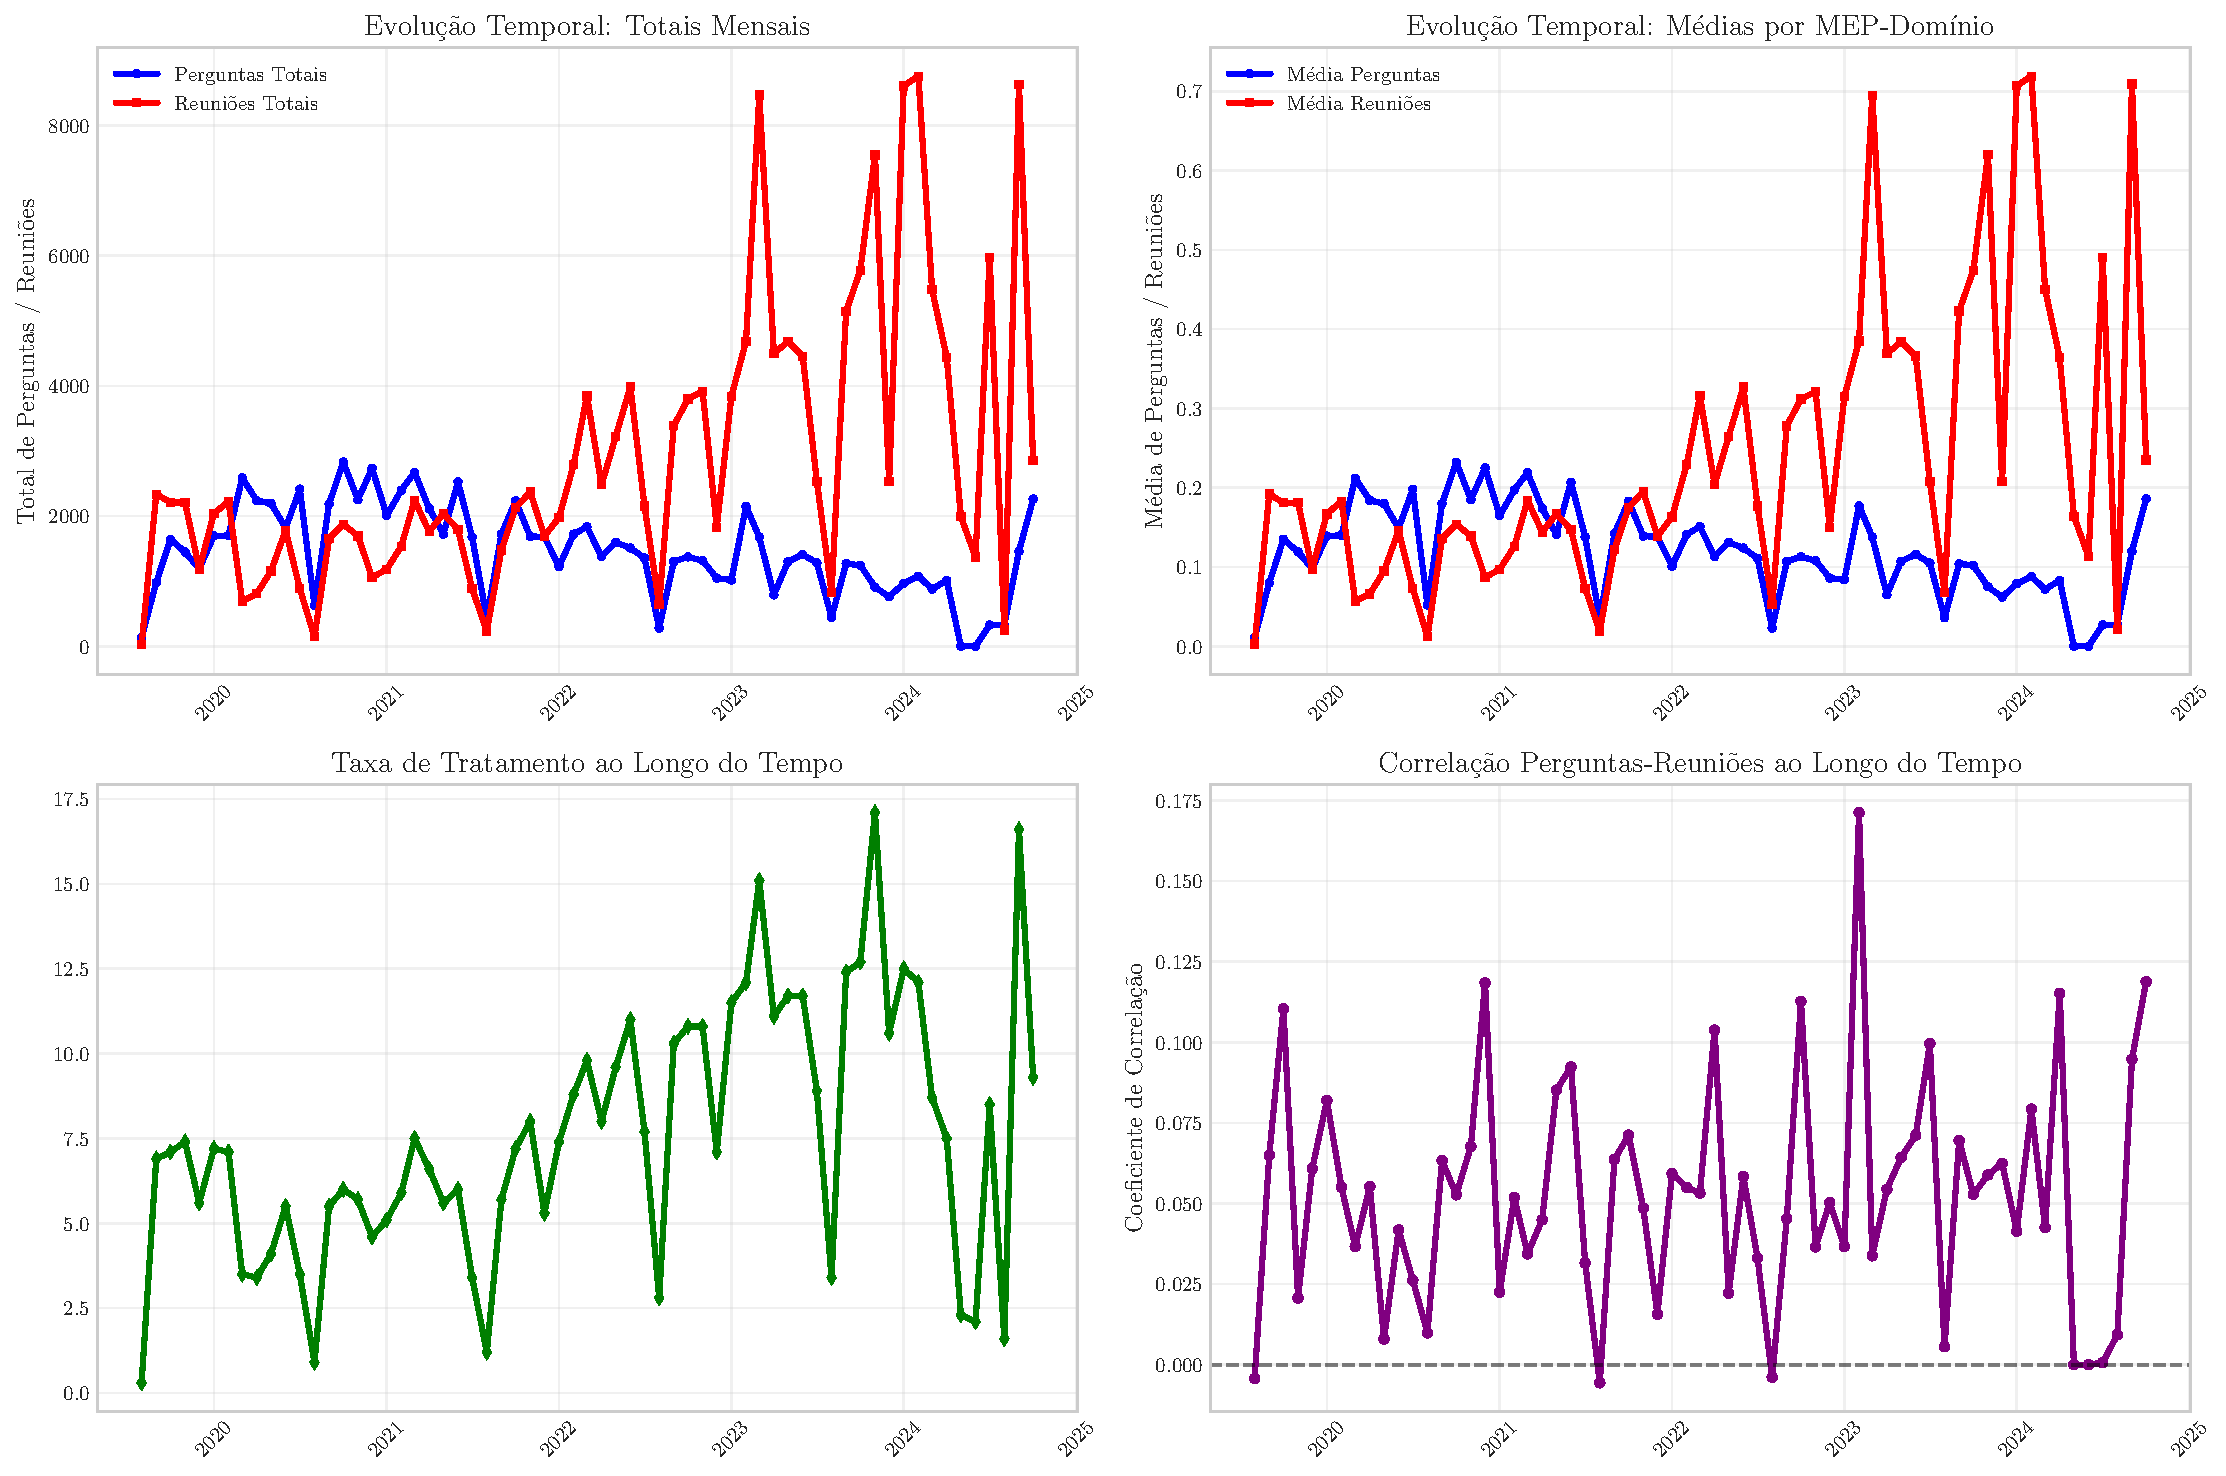
\includegraphics[width=\textwidth]{figures/fig2_time_series_analysis.pdf}
\caption{Evolução temporal da atividade parlamentar e de lobbying}
\label{fig:time_series}
\note{O painel superior esquerdo mostra os totais mensais agregados de perguntas e reuniões. O painel superior direito apresenta as médias mensais por observação MEP-domínio. O painel inferior esquerdo mostra a evolução da proporção de observações com atividade de lobbying. O painel inferior direito apresenta a estabilidade da correlação contemporânea entre as variáveis ao longo do tempo.}
\end{figure}

A análise temporal revela quatro padrões empiricamente relevantes. Primeiro, observa-se uma \textbf{tendência crescente} em ambas as variáveis ao longo do período, sugerindo intensificação tanto da atividade parlamentar quanto do lobbying. Segundo, existe clara \textbf{sazonalidade} relacionada ao calendário parlamentar, com reduções sistemáticas durante períodos de recesso. Terceiro, identificam-se \textbf{picos de atividade} que coincidem com discussões de legislação relevante em domínios específicos, indicando resposta coordenada do sistema político. Quarto, a \textbf{correlação contemporânea} entre perguntas e reuniões permanece relativamente estável ao longo do tempo, sugerindo estabilidade estrutural na relação entre as variáveis.

% não há exatamente essa tendência cerescente...


Estes padrões temporais têm implicações metodológicas importantes. A presença de tendências temporais justifica a inclusão de efeitos fixos de tempo nas especificações econométricas para controlar choques temporais comuns. A sazonalidade observada valida a escolha da frequência mensal como unidade temporal, capturando variações de curto prazo sem introduzir ruído excessivo. A estabilidade da correlação fornece evidência preliminar contra quebras estruturais que poderiam comprometer a validade das estimativas.

% \subsection{Padrões de participação: análise agregada por deputado}

Complementando a análise temporal, é fundamental examinar os padrões de participação no nível individual dos deputados. Esta perspectiva agregada revela a distribuição da atividade de lobbying entre os parlamentares e fornece insights sobre a concentração e heterogeneidade dos fenômenos estudados.

\subsubsection{Distribuição do tratamento entre deputados}

A \autoref{fig:mep_aggregated} apresenta uma análise abrangente dos padrões de participação agregados por deputado, revelando aspectos fundamentais da distribuição da atividade de lobbying no Parlamento Europeu.

\begin{figure}[htbp]
\centering
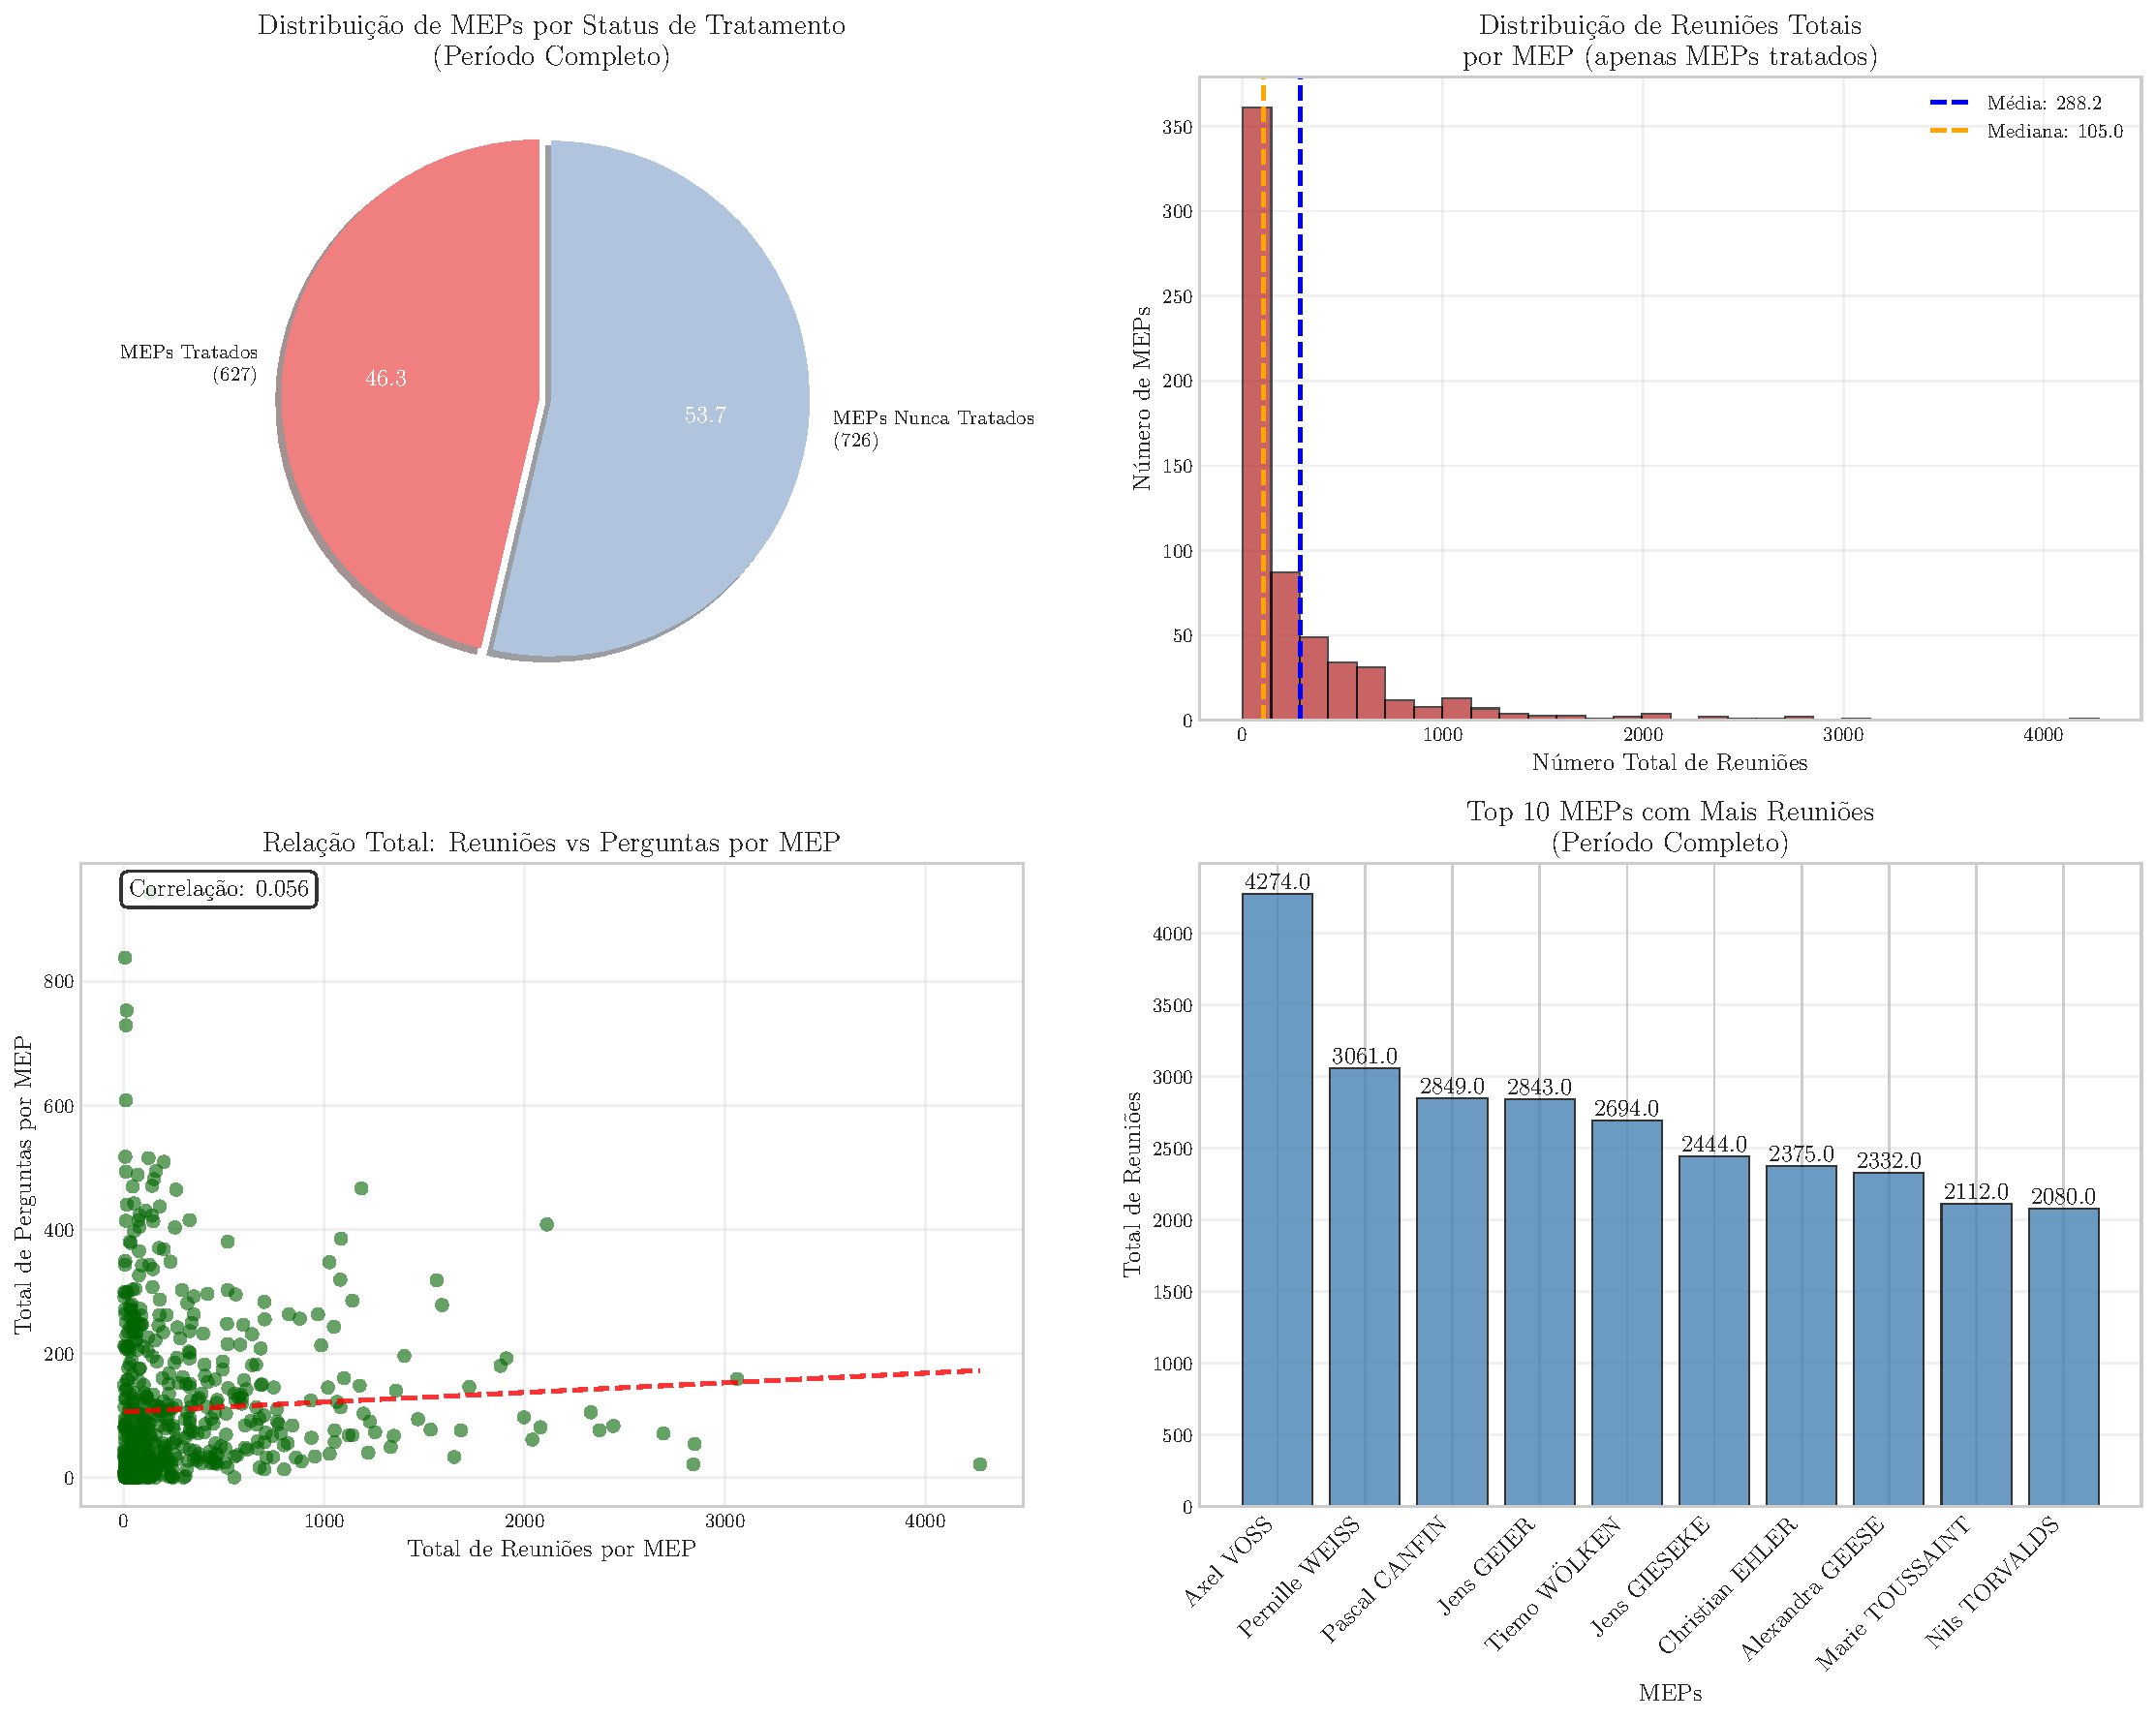
\includegraphics[width=\textwidth]{figures/fig6_mep_aggregated_analysis.pdf}
\caption{Análise agregada por MEP: distribuição e intensidade do tratamento}
\label{fig:mep_aggregated}
\note{O painel superior esquerdo mostra a proporção de deputados que receberam pelo menos uma reunião de lobbying durante todo o período. O painel superior direito apresenta a distribuição da intensidade total de reuniões entre deputados tratados. O painel inferior esquerdo examina a relação agregada entre reuniões e perguntas totais por deputado. O painel inferior direito identifica os deputados mais ativos em termos de recepção de lobbying.}
\end{figure}

A análise revela três características fundamentais da distribuição de tratamento. Primeiro, existe \textbf{participação substancial mas não universal}: 46,3\% dos deputados (627 de 1.353) receberam pelo menos uma reunião de lobbying durante o período estudado. Esta proporção indica que o lobbying é um fenômeno disseminado mas não ubíquo no sistema parlamentar europeu.

Segundo, observa-se \textbf{concentração extrema} na intensidade de tratamento. Entre os deputados que receberam lobbying, a distribuição é altamente assimétrica: enquanto a mediana é de 105 reuniões por deputado, a média é de 288,2 reuniões, indicando que uma minoria de parlamentares concentra uma proporção desproporcional da atividade lobista. O caso extremo de um deputado com 4.274 reuniões ilustra esta concentração.

Terceiro, a \textbf{correlação agregada} entre reuniões e perguntas totais por deputado é surpreendentemente baixa (0,056), contrastando com correlações mais elevadas observadas no nível temporal. Este padrão sugere que os efeitos do lobbying podem ser mais evidentes em frequências temporais específicas do que em padrões de atividade agregados de longo prazo.

% \paragraph{Implicações para a estratégia empírica}

Estes padrões agregados têm implicações importantes para a identificação causal. A concentração do tratamento em uma minoria de deputados sugere que estratégias de identificação baseadas em variação cross-sectional podem sofrer de poder estatístico limitado. Simultaneamente, a variação substancial na intensidade de tratamento entre deputados tratados fornece fonte valiosa de identificação para estimativas de dose-resposta.

A baixa correlação agregada, combinada com correlações temporais mais elevadas, indica que a identificação causal pode beneficiar-se de estratégias que explorem variação temporal within-individual rather than cross-sectional between-individual. Esta evidência preliminar orienta a especificação de modelos com efeitos fixos de deputado para controlar heterogeneidade não observada time-invariant.

\begin{table}[htbp]
\centering
\caption{Estatísticas agregadas de tratamento por deputado}
\label{tab:mep_treatment_stats}
\begin{tabular}{lr}
\toprule
\textbf{Estatística} & \textbf{Valor} \\
\midrule
Total de deputados únicos & 1{,}353 \\
Deputados que receberam tratamento & 627 \\
Taxa de tratamento por deputado (\%) & 46{,}3\% \\
\midrule
\textbf{Entre deputados tratados:} & \\
Reuniões médias por deputado & 288{,}2 \\
Reuniões medianas por deputado & 105{,}0 \\
Desvio padrão & 468{,}9 \\
Deputado mais ativo (reuniões) & 4{,}274 \\
\midrule
\textbf{Correlação agregada:} & \\
Correlação reuniões-perguntas & 0{,}056 \\
\bottomrule
\end{tabular}
\end{table}

\subsection{Heterogeneidade entre domínios de política pública}

A terceira dimensão da análise agregada examina a variação entre domínios de política pública. Esta heterogeneidade setorial é teoricamente relevante porque diferentes áreas de política podem apresentar características distintas em termos de complexidade técnica, interesse econômico e organização de grupos de pressão, afetando tanto a demanda por lobbying quanto a responsividade parlamentar.

% \paragraph{Padrões de tratamento por domínio}

A \autoref{fig:domain_treatment} apresenta uma análise sistemática da variação inter-domínios em múltiplas dimensões: penetração, volume e intensidade do tratamento, bem como padrões temporais de iniciação.


\begin{table}[htbp]
    \centering
    \caption{Taxa de tratamento por domínio: deputados únicos que receberam lobbying}
    \label{tab:domain_treatment_rates}
    \begin{tabular}{lrrr}
    \toprule
    \textbf{Domínio} & \textbf{Deputados Tratados} & \textbf{Total Deputados} & \textbf{Taxa (\%)} \\
    \midrule
    Economia e Comércio & 615 & 1{,}353 & 45{,}5 \\
    Tecnologia & 615 & 1{,}353 & 45{,}5 \\
    Política Externa e Segurança & 611 & 1{,}353 & 45{,}2 \\
    Infraestrutura e Indústria & 610 & 1{,}353 & 45{,}1 \\
    Meio Ambiente e Clima & 607 & 1{,}353 & 44{,}9 \\
    Saúde & 599 & 1{,}353 & 44{,}3 \\
    Educação & 578 & 1{,}353 & 42{,}7 \\
    Direitos Humanos & 564 & 1{,}353 & 41{,}7 \\
    Agricultura & 554 & 1{,}353 & 40{,}9 \\
    \bottomrule
    \end{tabular}
    \end{table}

A análise revela heterogeneidade sistemática mas moderada entre domínios. Em termos de \textbf{penetração}, as taxas variam de 40,9\% (agricultura) a 45,5\% (economia e tecnologia), uma amplitude de apenas 4,6 pontos percentuais. Esta variação relativamente pequena sugere que o lobbying possui caráter transversal, não concentrando-se drasticamente em setores específicos.

Contudo, emergem padrões teoricamente consistentes. Domínios relacionados à \textbf{regulação econômica} (economia e comércio, tecnologia, infraestrutura) apresentam sistematicamente maiores taxas de penetração, refletindo os elevados interesses econômicos e a complexidade regulatória que incentivam investimento em atividades de lobbying. Este padrão é especialmente relevante considerando que a promoção da integração econômica é o foco principal de um bloco como a União Europeia, o que naturalmente direciona maior atenção e mobilização de grupos de interesse para essas áreas. Inversamente, domínios com características de bem público (agricultura, direitos humanos) apresentam menores taxas, consistente com problemas de ação coletiva e menor capacidade organizacional de grupos difusos.


\begin{figure}[htbp]
    \centering
    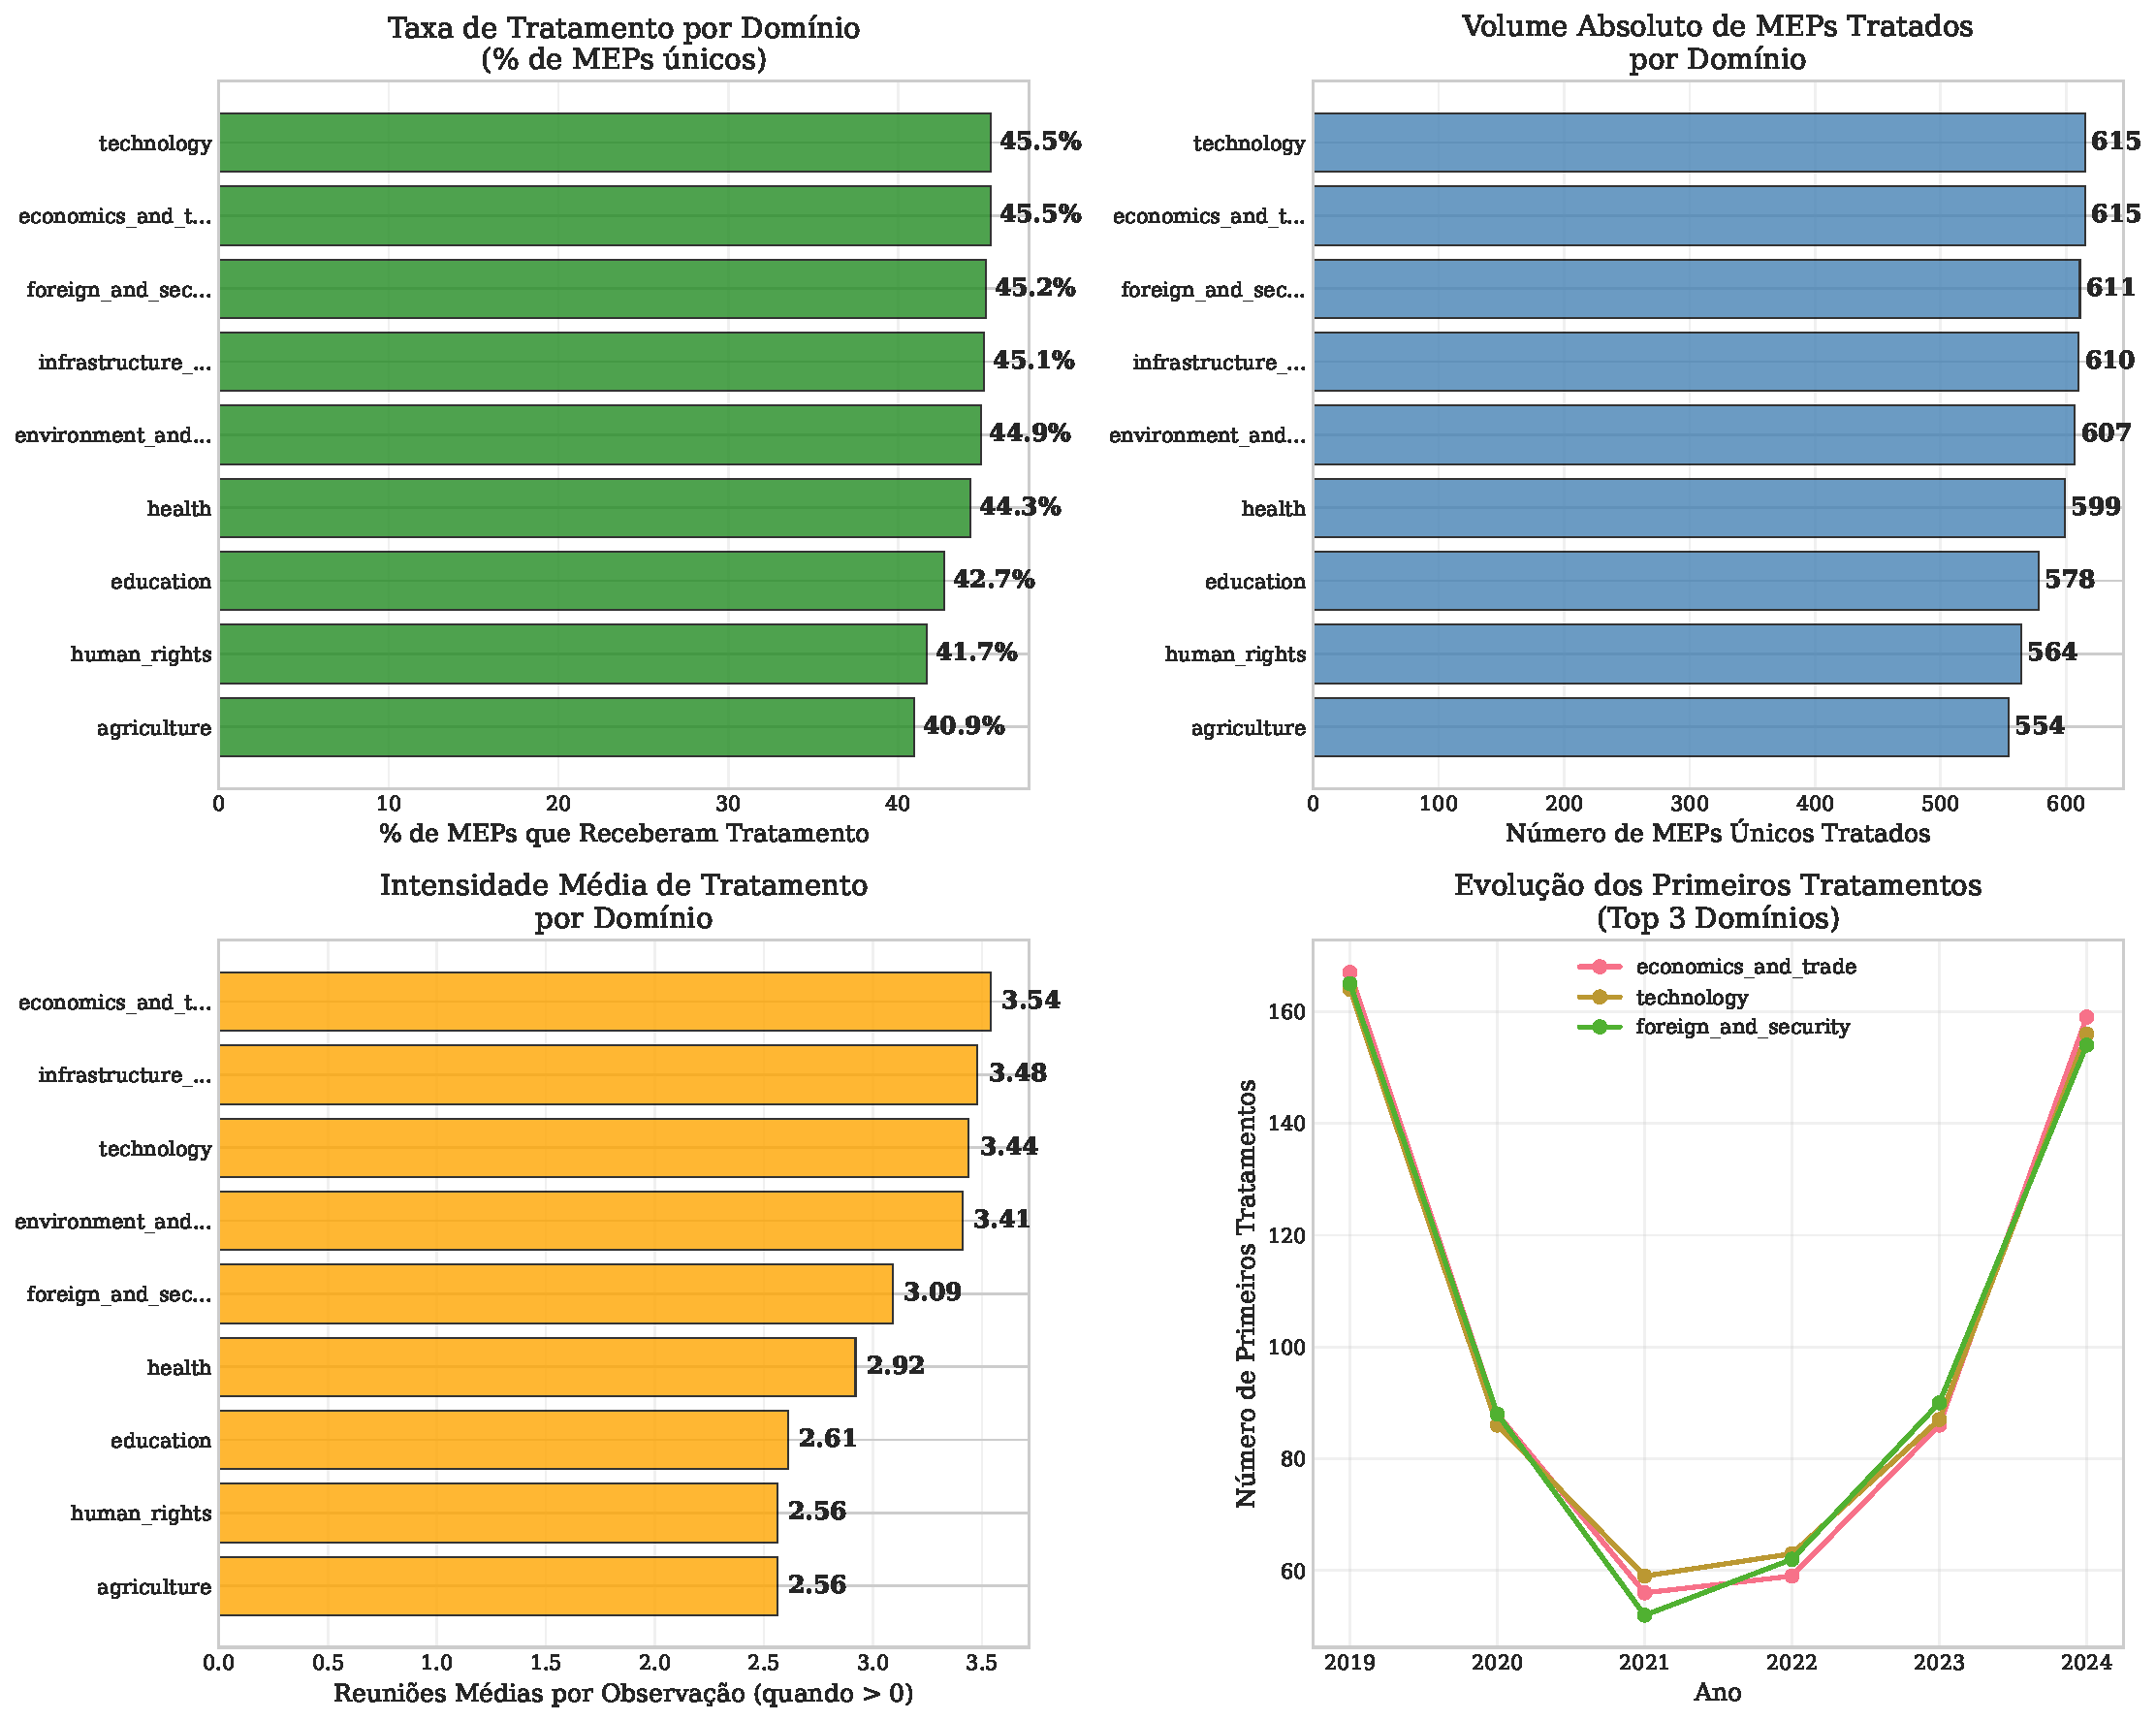
\includegraphics[width=\textwidth]{figures/fig7_domain_treatment_analysis.pdf}
    \caption{Análise detalhada de tratamento por domínio de política pública}
    \label{fig:domain_treatment}
    \note{O painel superior esquerdo mostra a taxa de penetração (percentual de deputados únicos que receberam pelo menos uma reunião em cada domínio). O painel superior direito apresenta o volume absoluto de deputados tratados. O painel inferior esquerdo mostra a intensidade média condicional de tratamento. O painel inferior direito apresenta a evolução temporal dos primeiros tratamentos para os três domínios mais ativos.}
\end{figure}


A heterogeneidade observada entre domínios tem duas implicações metodológicas importantes. Primeiro, a variação sistemática sugere que estimativas de efeito médio podem mascarar diferenças substantivas entre setores, justificando análises de heterogeneidade de efeitos por domínio. Segundo, a ordenação consistente dos domínios por múltiplas métricas (penetração, volume, intensidade) sugere que esta heterogeneidade reflete características estruturais dos setores ao invés de variação aleatória, aumentando a credibilidade de interpretações causais diferenciadas.

% \begin{figure}[htbp]
% \centering
% 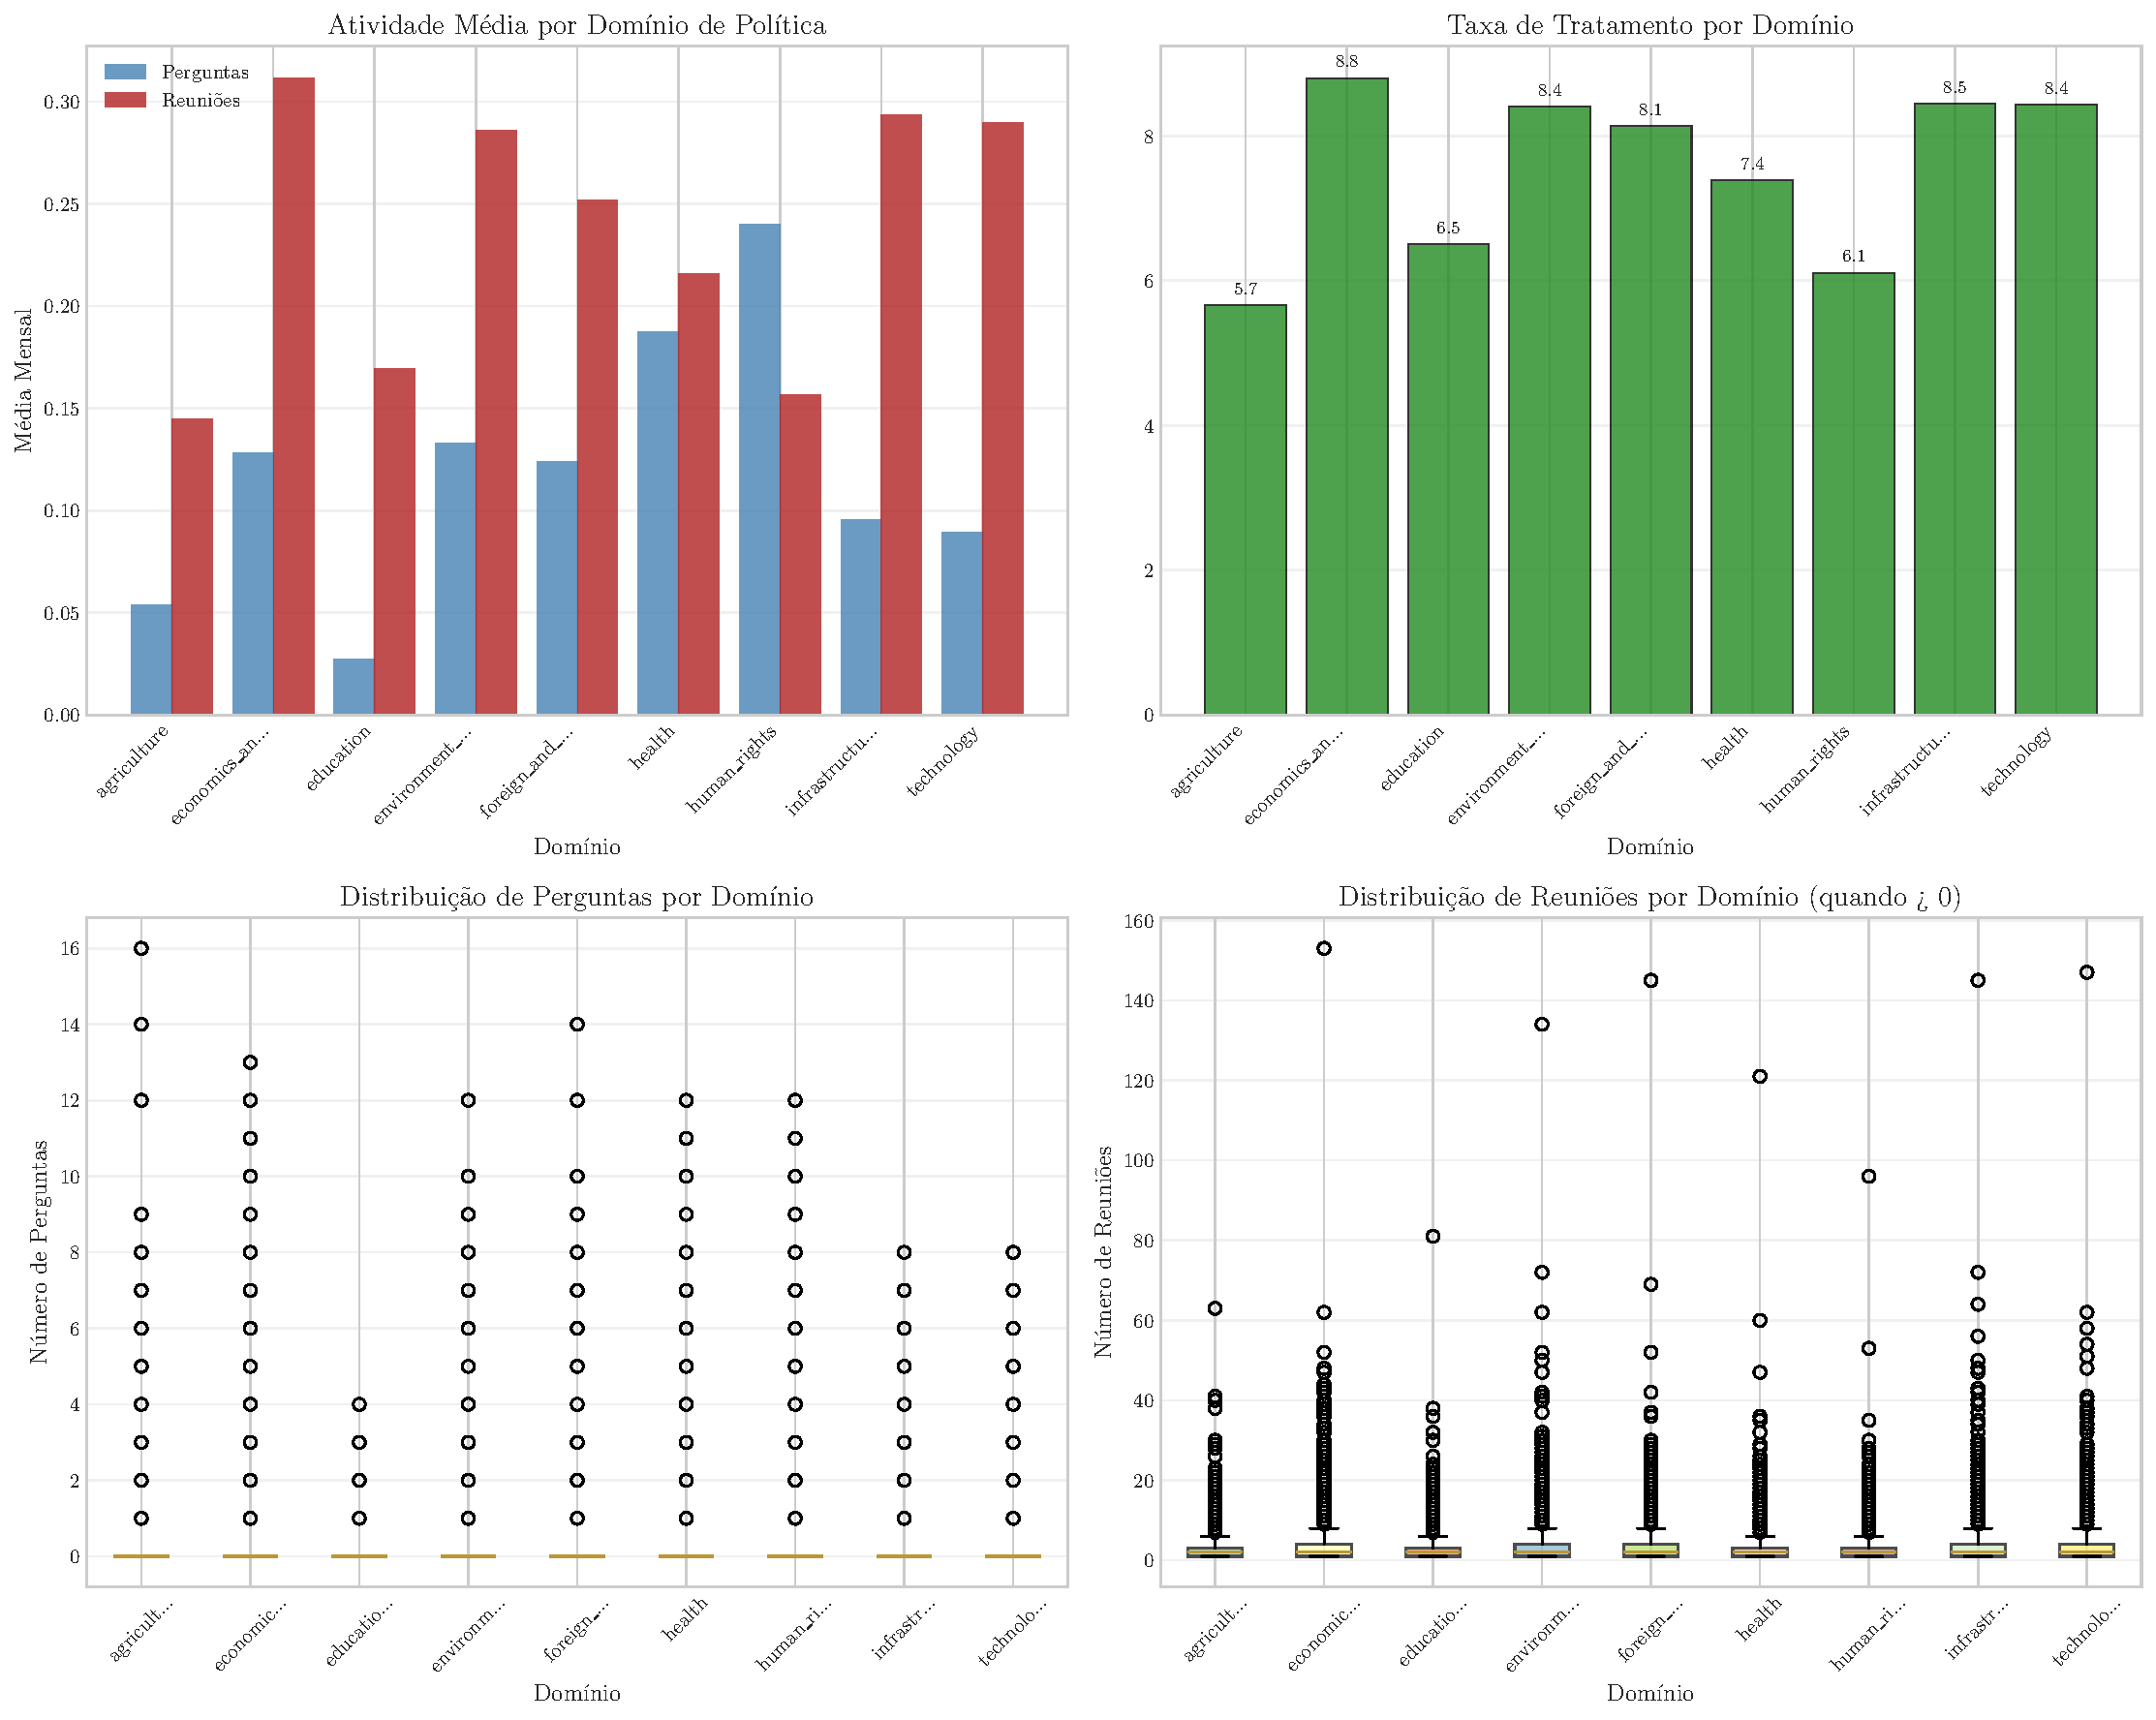
\includegraphics[width=.9\textwidth]{figures/fig3_domain_heterogeneity.pdf}
% \caption{Heterogeneidade por domínio: atividade média e distribuições}
% \label{fig:domain_heterogeneity}
% \note{O painel superior esquerdo mostra a atividade média mensal por domínio para ambas as variáveis. O painel superior direito apresenta as taxas de tratamento mensais. Os painéis inferiores mostram box plots das distribuições completas por domínio, evidenciando tanto diferenças de localização quanto de dispersão entre áreas de política pública.}
% \end{figure}

% \subsection{Análise detalhada: observações MEP-domínio-período}

% Após estabelecer os padrões agregados gerais, temporais e setoriais, esta seção examina as características específicas dos dados no nível mais desagregado: observações MEP-domínio-mês. Esta análise é crucial porque a unidade de observação constitui a base para as estimações econométricas e suas características distribucionais determinam as escolhas metodológicas apropriadas.

% \paragraph{Especialização temática e o problema da inflação artificial de zeros}

A análise da inflação de zeros requer cuidado metodológico particular, pois a unidade de observação MEP-domínio-mês pode gerar inflação \textbf{artificial} de zeros. Como documentado na literatura sobre comportamento parlamentar \cite{example}, deputados tendem a especializar-se tematicamente, concentrando atividade em subconjuntos específicos de domínios. Consequentemente, grupos de interesse, cientes desta especialização, direcionam esforços de lobbying apenas para deputados ativos em suas áreas de interesse.

\textbf{Evidência de especialização temática:} A análise da atividade parlamentar agregada por deputado revela que 97,6\% dos MEPs são \textbf{generalistas} (Índice Herfindahl < 0,4), atuando em média em 7,47 dos 9 domínios disponíveis. Contudo, identificam-se 22 MEPs altamente especializados (HHI > 0,8) que concentram perguntas em domínios únicos, e 26 moderadamente especializados (HHI 0,4-0,8), demonstrando que a especialização, embora limitada, é empiricamente relevante.

\paragraph{Análise corrigida da inflação de zeros}

Para evitar viés na interpretação, a análise da inflação de zeros deve considerar níveis de agregação teoricamente apropriados. A \autoref{tab:zero_inflation_comparison} apresenta uma comparação sistemática entre diferentes níveis de agregação.

\begin{table}[htbp]
\centering
\caption{Inflação de zeros por nível de agregação}
\label{tab:zero_inflation_comparison}
% Usar tabularx para permitir quebra de linha na primeira coluna e evitar overfull hbox
\begin{tabularx}{\textwidth}{>{\raggedright\arraybackslash}X r r r}
\toprule
\textbf{Nível de Agregação} & \textbf{Observações} & \textbf{Zeros Perguntas} & \textbf{Zeros Reuniões} \\
\midrule
MEP-Domínio-Mês (original) & 767{.}151 & 92{,}2\% & 92{,}5\% \\
MEP-Mês (domínios ativos) & 54{.}117 & 70{,}9\% & 85{,}2\% \\
Domínio-Mês (agregado) & 567 & 3{,}2\% & 0{,}0\% \\
\bottomrule
\end{tabularx}
\end{table}

Os resultados revelam que a inflação de zeros é \textbf{sensível ao nível de agregação} e parcialmente \textbf{artificial} quando consideramos especializações temáticas:

\begin{enumerate}
    \item \textbf{Nível MEP-domínio-mês}: A inflação aparentemente extrema (>92\%) reflete em grande parte combinações MEP-domínio onde não se espera atividade sistemática devido à especialização.
    
    \item \textbf{Nível MEP-mês} (agregando apenas domínios onde o MEP demonstra atividade parlamentar): A inflação reduz substancialmente para 70,9\% (perguntas) e 85,2\% (reuniões), revelando que a atividade é \textit{episódica} mas não \textit{ausente}.
    
    \item \textbf{Nível domínio-mês} (agregando todos os MEPs ativos): A inflação torna-se negligível (3,2\% para perguntas, 0\% para reuniões), indicando que há atividade consistente em todos os domínios quando consideramos o conjunto de deputados relevantes.
\end{enumerate}

% A \autoref{fig:corrected_zero_inflation} apresenta uma comparação visual sistemática entre os diferentes níveis de agregação, evidenciando como a especialização temática afeta a interpretação da inflação de zeros.

% \begin{figure}[htbp]
% \centering
% 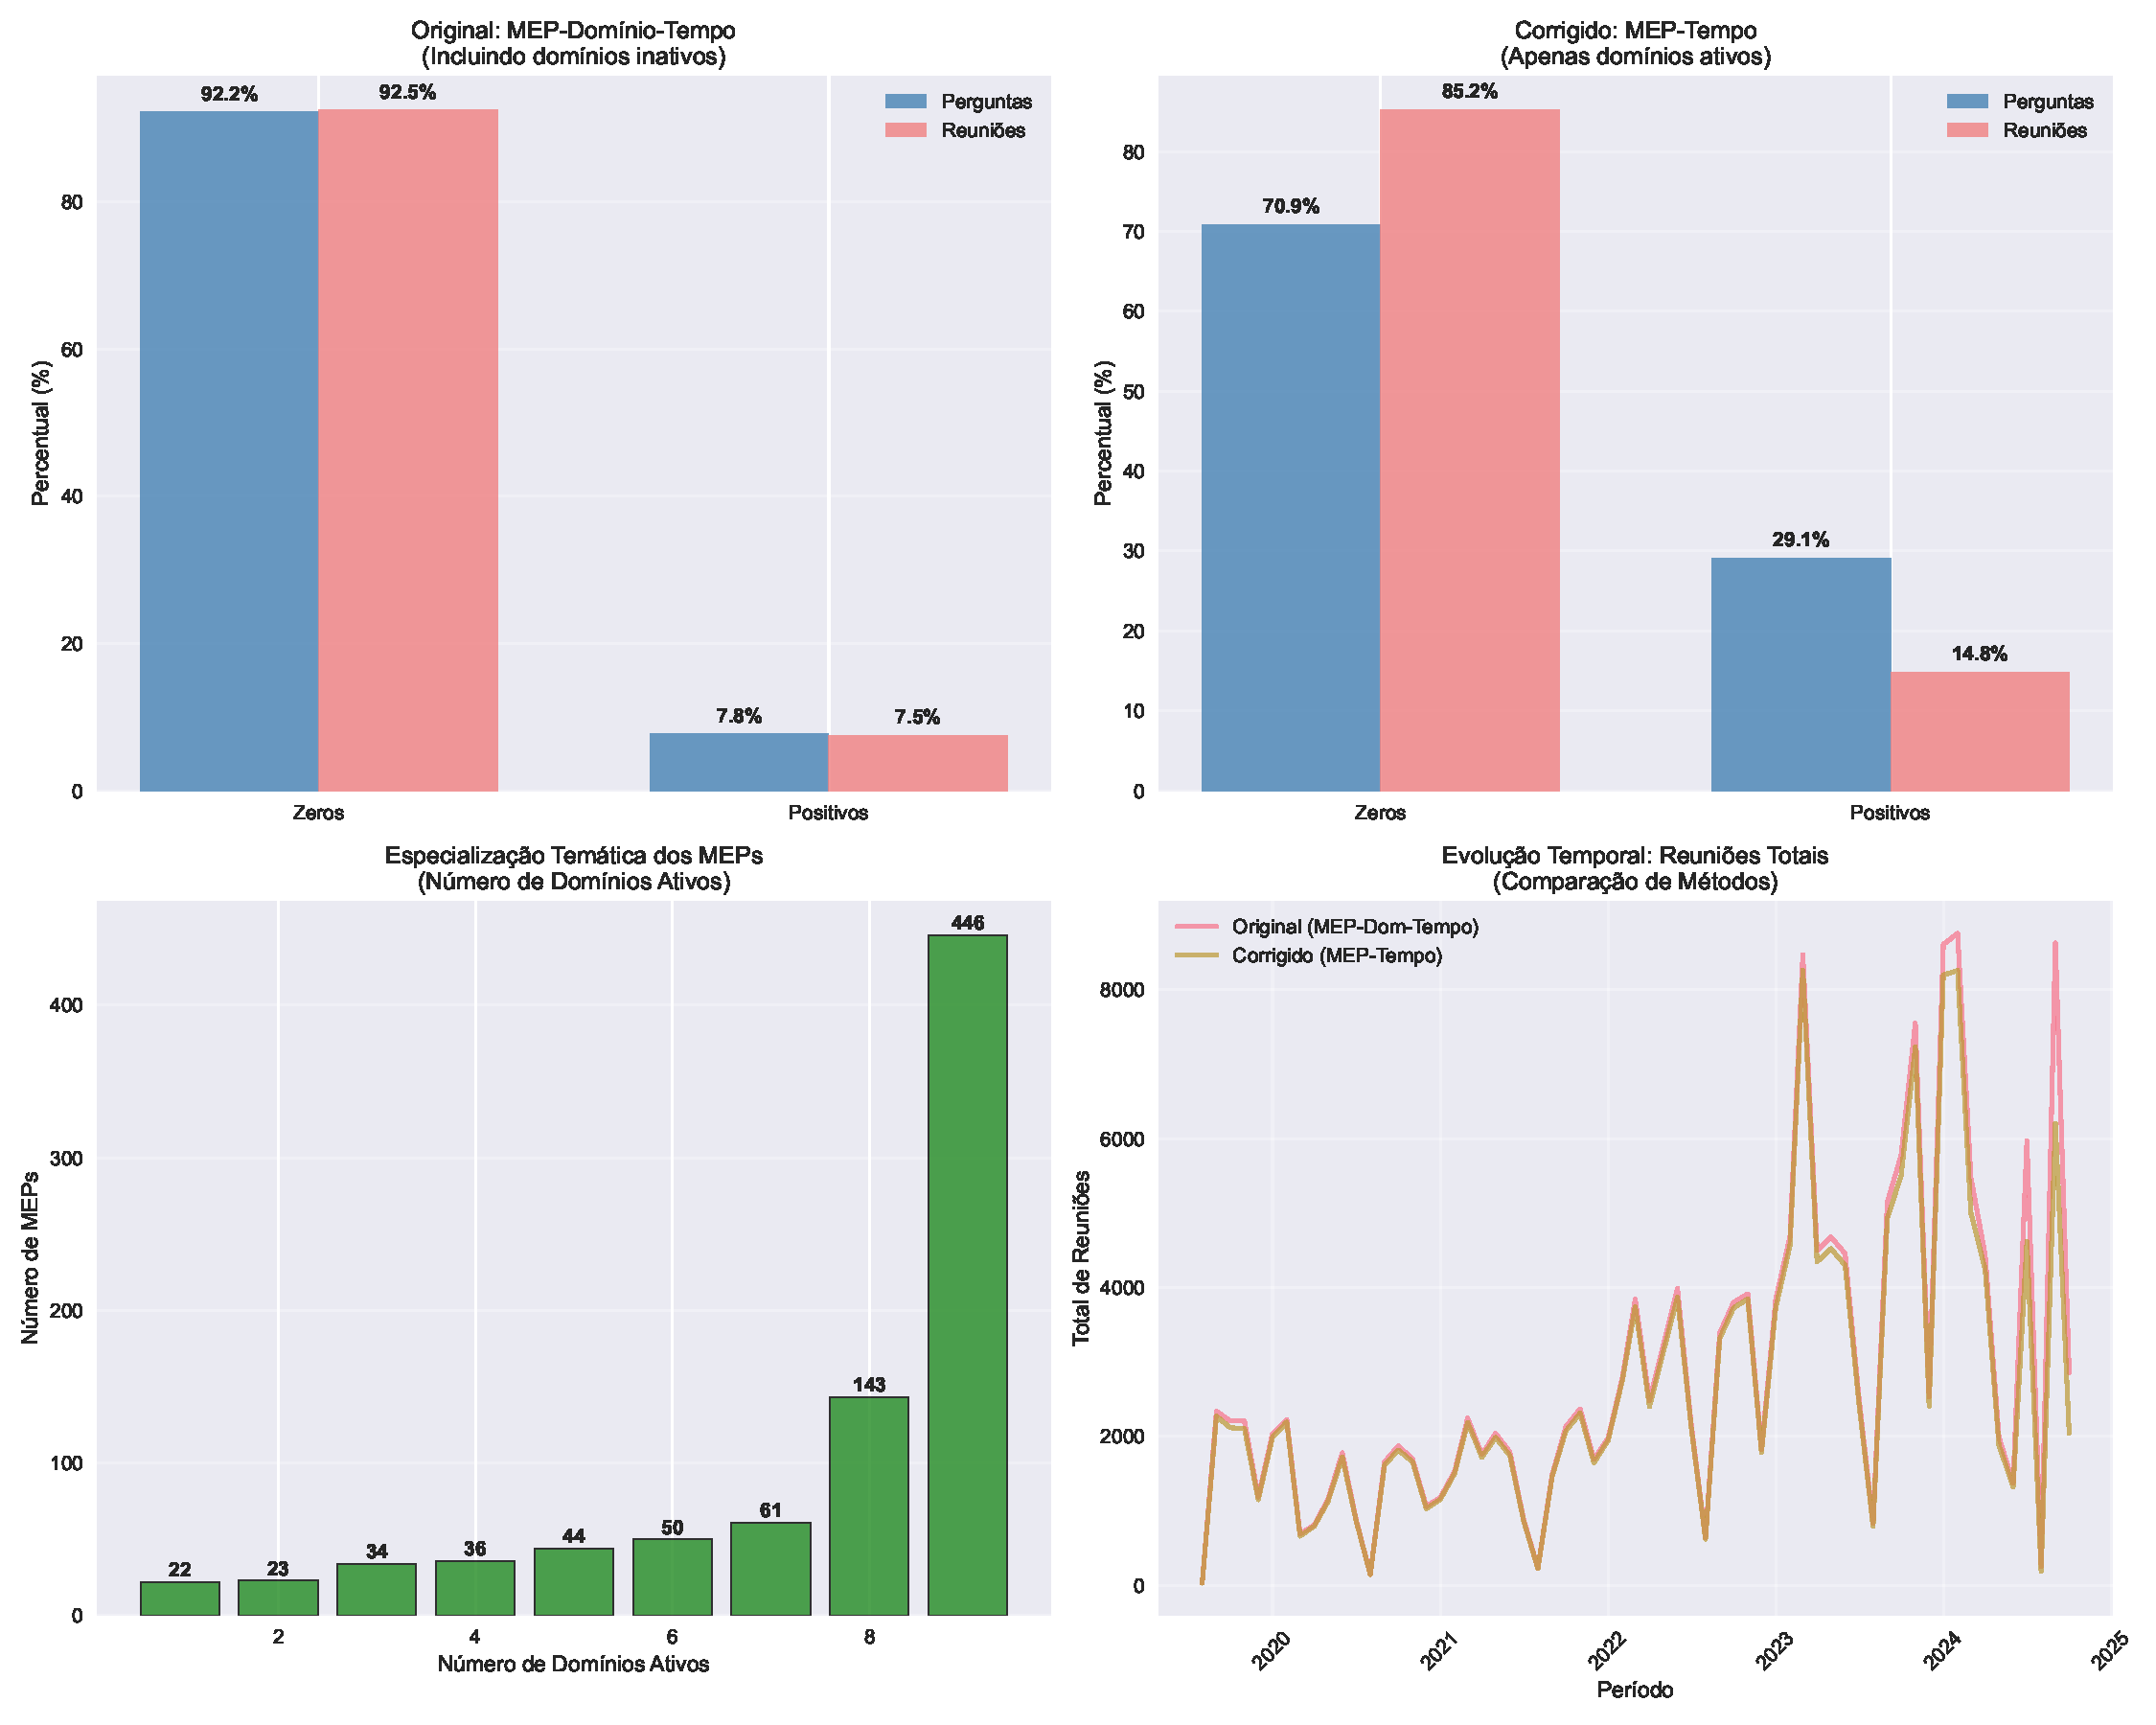
\includegraphics[width=\textwidth]{figures/fig_corrected_zero_inflation_analysis.pdf}
% \caption{Análise corrigida da inflação de zeros considerando especialização temática}
% \label{fig:corrected_zero_inflation}
% \note{O painel superior esquerdo mostra a inflação aparente no nível MEP-domínio-mês original. O painel superior direito apresenta a inflação corrigida no nível MEP-mês considerando apenas domínios ativos. O painel inferior esquerdo mostra a distribuição de especialização temática dos MEPs. O painel inferior direito compara a evolução temporal dos totais mensais entre os métodos original e corrigido.}
% \end{figure}

% \paragraph{Implicações metodológicas revisadas}

Esta análise corrigida tem implicações fundamentais para a estratégia econométrica:

\begin{enumerate}
    \item \textbf{Falso problema de inflação de zeros}: A aparente inflação extrema (>92\%) é em grande parte \textbf{artificial}, resultante da inclusão de combinações MEP-domínio teoricamente implausíveis. A inflação \textbf{real} no nível MEP-mês é substancialmente menor (70,9\%-85,2\%).
    
    \item \textbf{Justificativa para efeitos fixos}: A especialização temática documentada justifica ainda mais fortemente o uso de efeitos fixos MEP×domínio, pois captura heterogeneidade não observada na propensão à atividade em áreas específicas.
    
    \item \textbf{Modelos econométricos apropriados}: Enquanto a inflação moderada (70,9\%) ainda sugere benefícios de modelos de contagem (PPML), a inflação não é tão extrema a ponto de requerer modelos zero-inflated especializados.
    
    \item \textbf{Unidade de análise}: A evidência sustenta a escolha da unidade MEP-domínio-mês para análise causal, pois captura a granularidade necessária para identificação, desde que acompanhada de controles apropriados para especialização.
    
    \item \textbf{Interpretação de resultados}: Efeitos estimados devem ser interpretados condicionalmente à especialização temática, com atenção particular às margens extensiva (entrada em novos domínios) versus intensiva (aumento de atividade em domínios existentes).
\end{enumerate}

% \paragraph{Decomposição em margens extensiva e intensiva}

% A extrema inflação de zeros torna analiticamente vantajoso decompor o fenômeno em duas margens conceituais distintas: a \textbf{margem extensiva} (decisão de participar) e a \textbf{margem intensiva} (nível de atividade condicional à participação). Esta decomposição é teoricamente relevante porque diferentes mecanismos causais podem operar em cada margem.

% A \autoref{fig:extensive_intensive} apresenta uma análise detalhada desta decomposição, incluindo a sobreposição entre atividades parlamentares e de lobbying.

% \begin{figure}[htbp]
% \centering
% 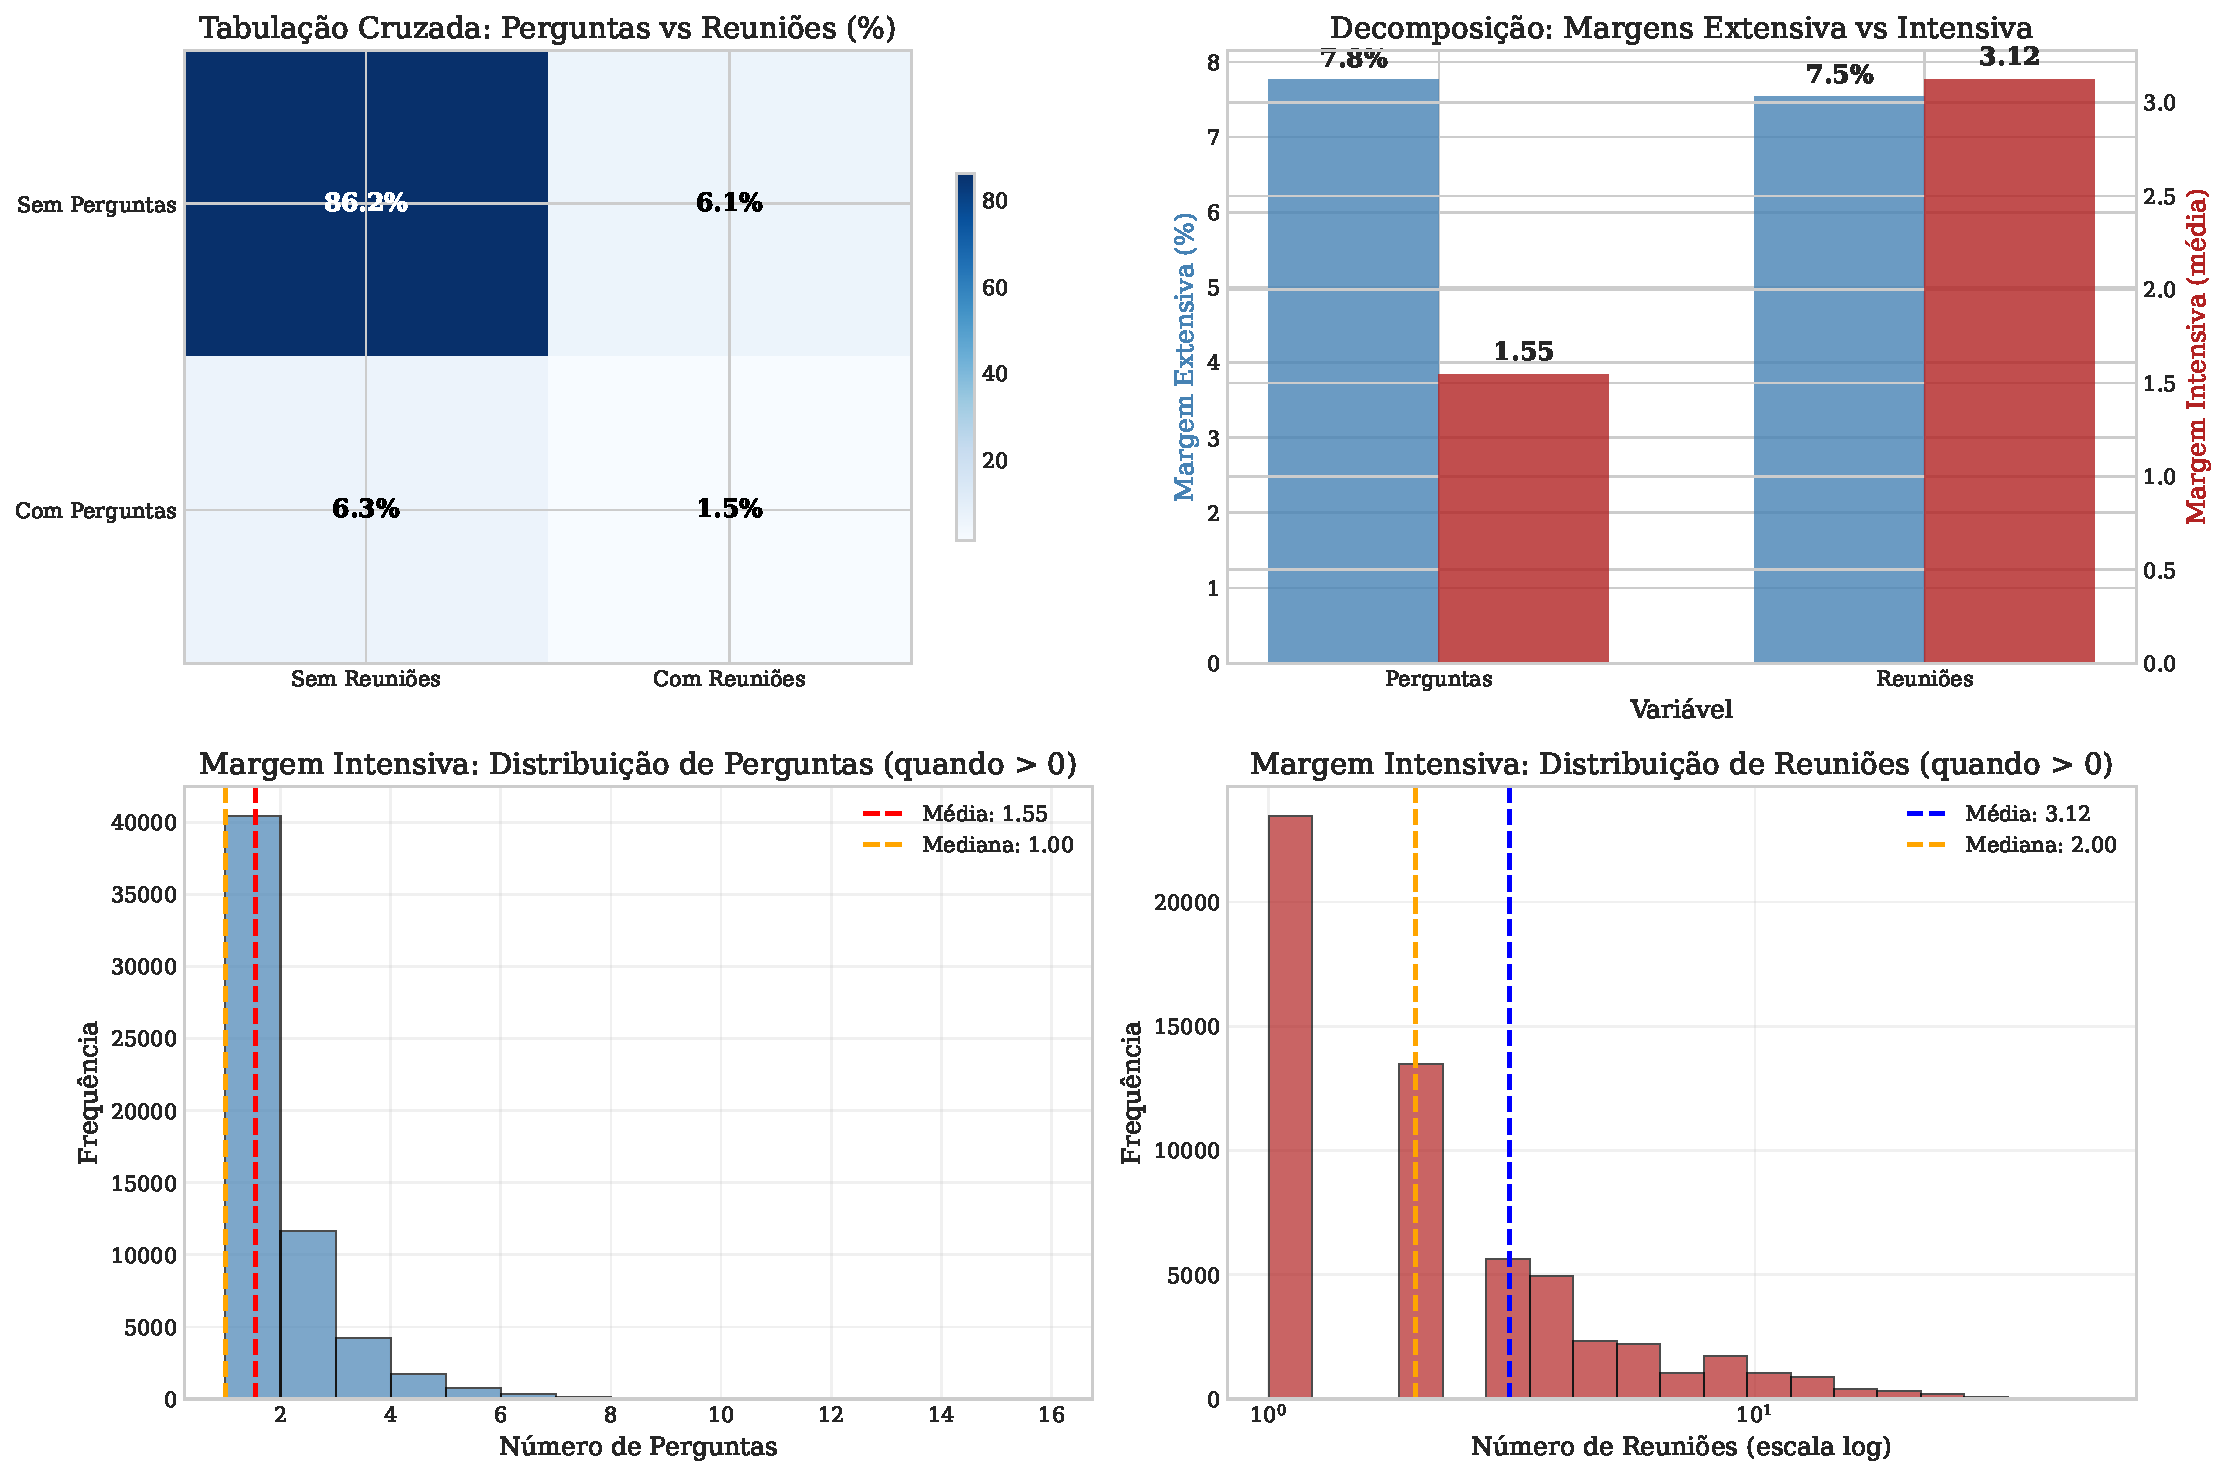
\includegraphics[width=\textwidth]{figures/fig5_extensive_intensive_margins.pdf}
% \caption{Análise das margens extensiva e intensiva}
% \label{fig:extensive_intensive}
% \note{O painel superior esquerdo apresenta a tabulação cruzada entre atividade parlamentar e de lobbying, revelando padrões de sobreposição. O painel superior direito decompõe as margens extensiva (participação) e intensiva (intensidade condicional). Os painéis inferiores mostram as distribuições condicionais completas para ambas as variáveis na margem intensiva.}
% \end{figure}

% A tabulação cruzada revela um padrão notável: apenas \textbf{0,4\%} das observações apresentam simultaneamente perguntas parlamentares e reuniões de lobbying. Esta baixa sobreposição indica que atividade parlamentar e lobbying são largamente \textbf{independentes} no nível temporal mensal, sugerindo que potenciais efeitos causais podem operar através de canais indiretos ou com defasagens temporais que não são captadas na correlação contemporânea.

% Na margem extensiva, 7,8\% das observações apresentam atividade parlamentar e 7,5\% apresentam atividade de lobbying. Na margem intensiva, condicionalmente à participação, as médias são 1,54 perguntas e 3,15 reuniões por observação, com distribuições altamente assimétricas evidenciando concentração mesmo dentro do subconjunto de observações ativas.

% \paragraph{Correlações e relações entre variáveis}

% Para completar a caracterização dos dados, a \autoref{fig:correlation_analysis} examina as relações diretas entre as variáveis principais através de múltiplas perspectivas analíticas.

% \begin{figure}[htbp]
% \centering
% 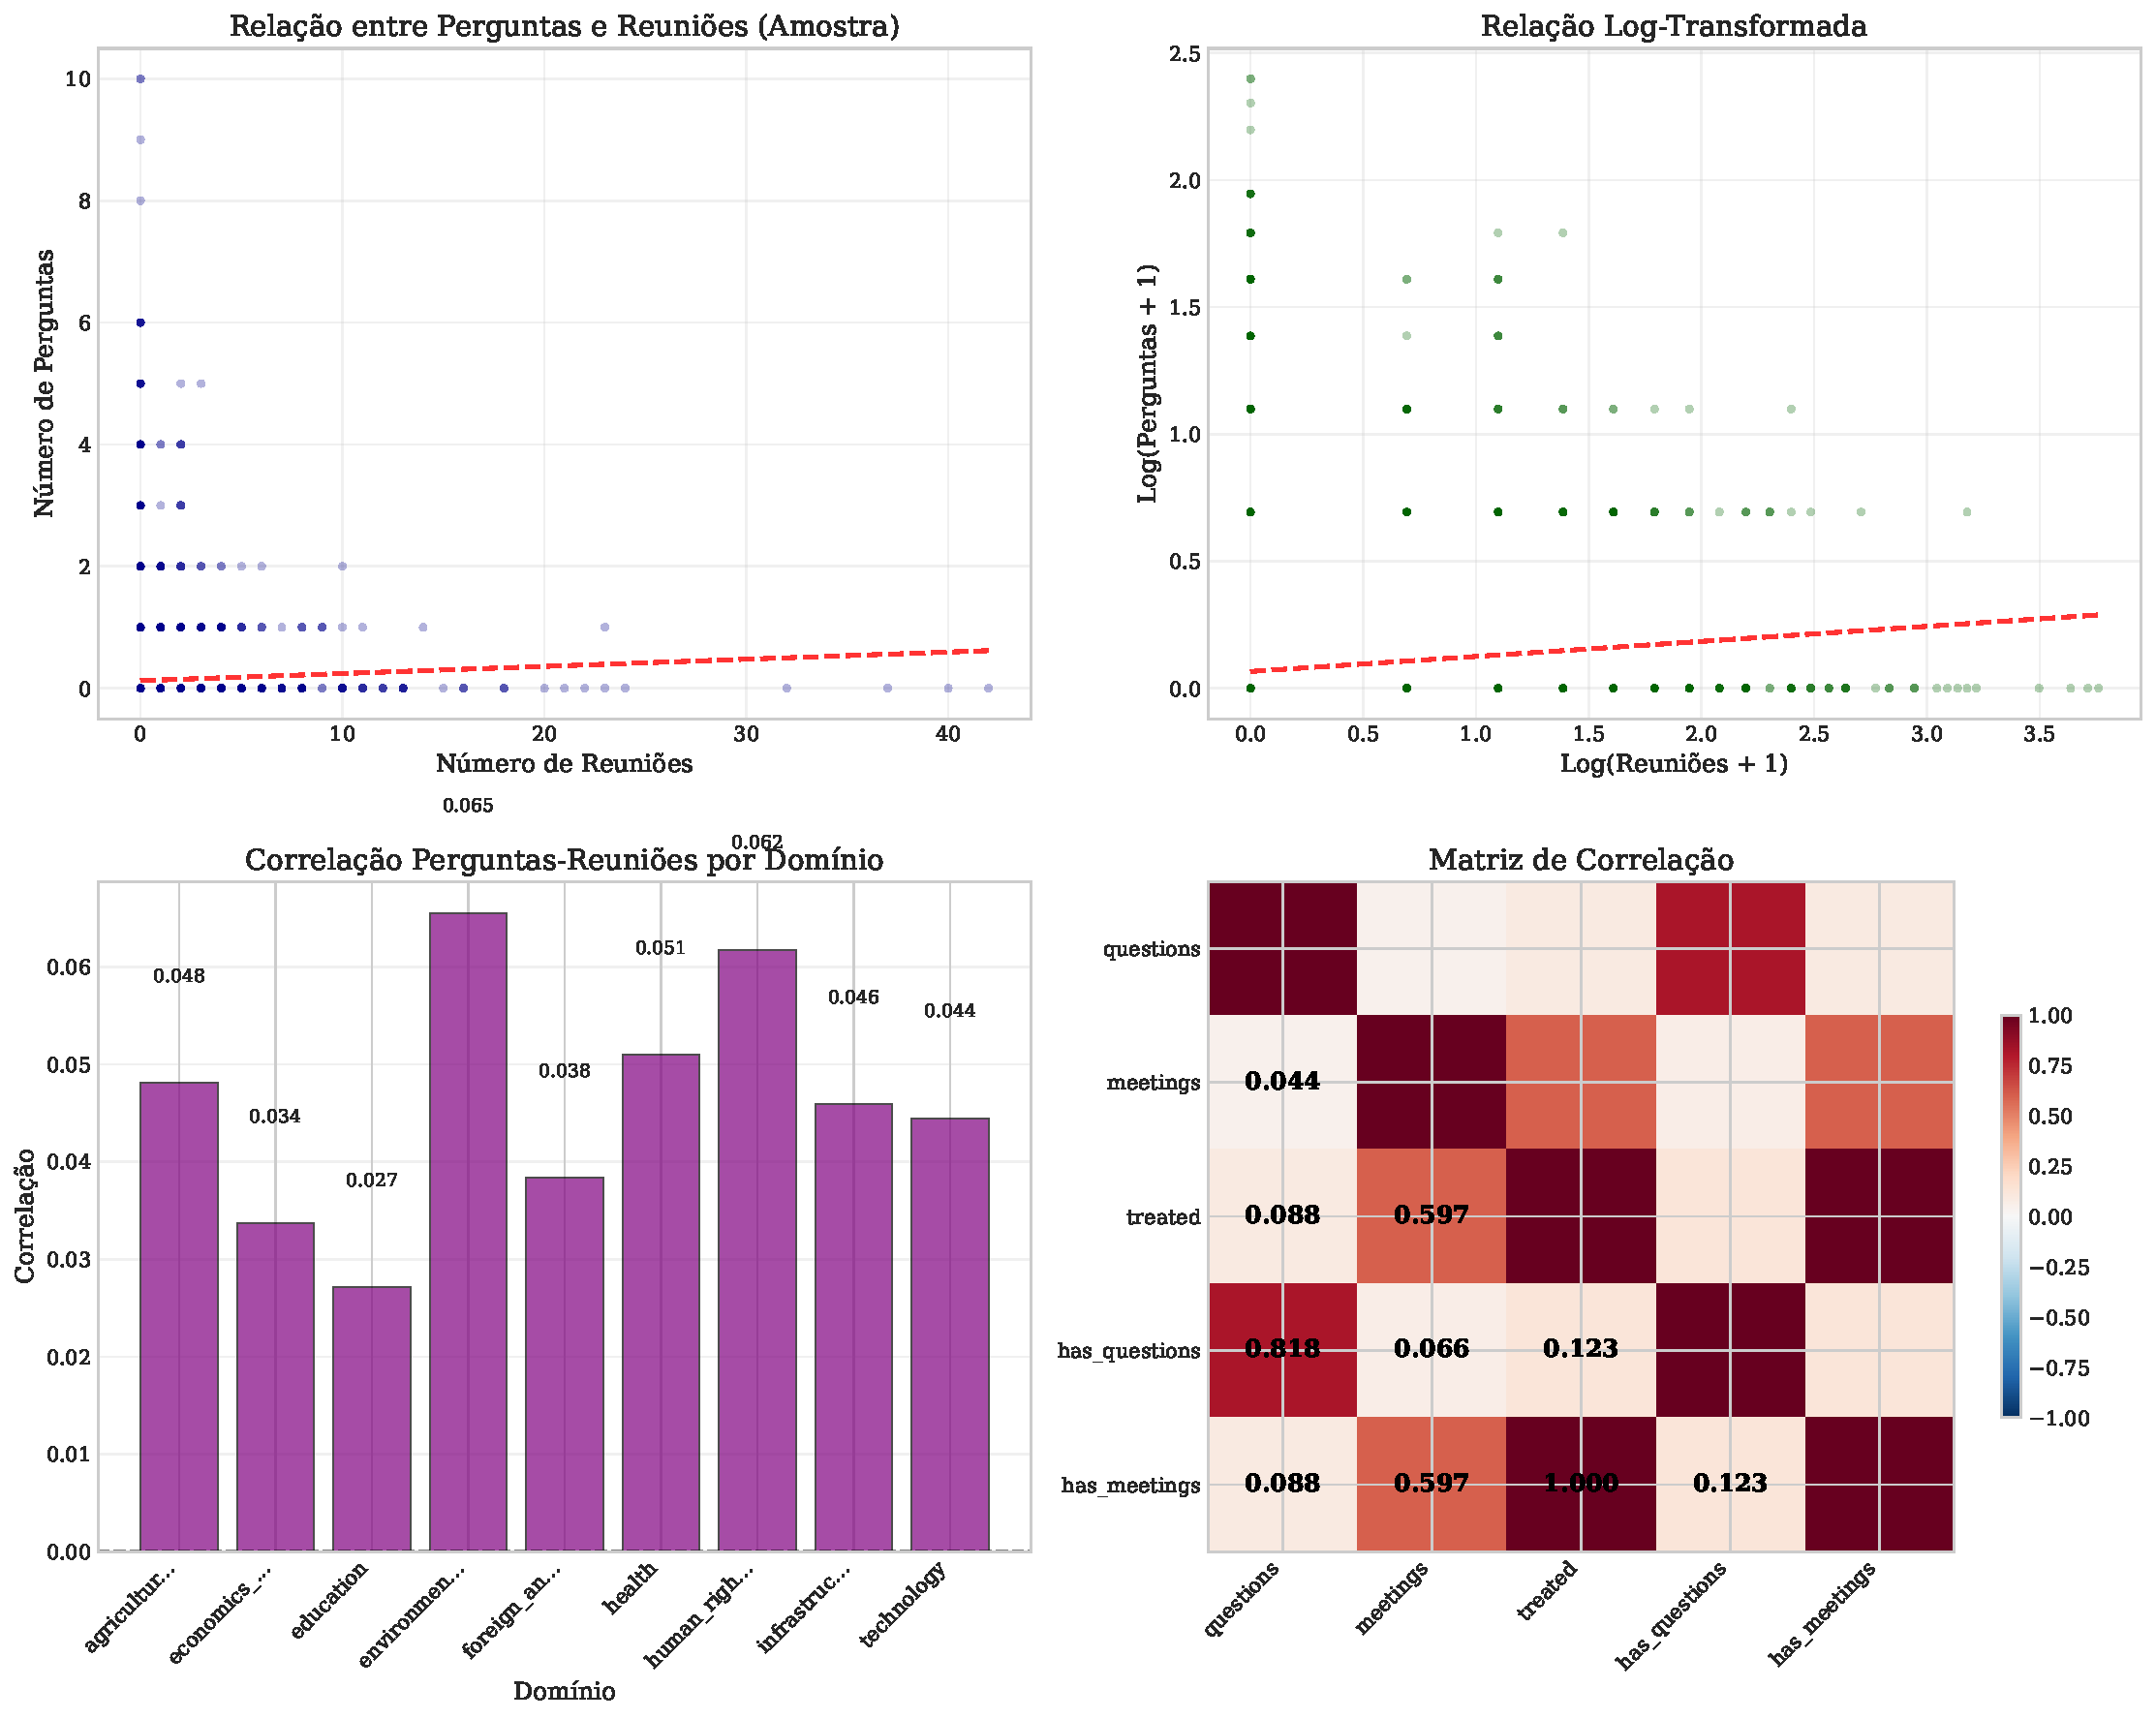
\includegraphics[width=\textwidth]{figures/fig4_correlation_analysis.pdf}
% \caption{Análise de correlações e relações entre variáveis}
% \label{fig:correlation_analysis}
% \note{O painel superior esquerdo mostra a relação geral entre perguntas e reuniões no nível MEP-domínio-mês. O painel superior direito apresenta a mesma relação em escala logarítmica. O painel inferior esquerdo mostra as correlações por domínio. O painel inferior direito apresenta a matriz de correlação entre as variáveis principais.}
% \end{figure}

% A análise de correlações revela padrões consistentes com a baixa sobreposição contemporânea observada anteriormente. No nível agregado MEP-domínio-mês, a correlação é positiva mas modesta. Interessantemente, existe heterogeneidade sistemática nas correlações entre domínios, sugerindo que a força da relação varia com características setoriais específicas.

\subsection{Síntese e implicações metodológicas}

A análise descritiva multinível revela um conjunto coerente de \textit{stylized facts} que informam tanto a compreensão teórica quanto as escolhas metodológicas para a análise causal subsequente.

% \paragraph{Características empíricas principais}

Primeiro, o \textbf{lobbying é um fenômeno disseminado mas episódico}. Enquanto 46,3\% dos deputados recebem lobbying durante o período estudado, a atividade temporal é concentrada: considerando apenas domínios onde MEPs demonstram atividade parlamentar, 70,9\% das observações MEP-mês não apresentam perguntas e 85,2\% não apresentam reuniões, indicando que a influência opera através de interações concentradas temporalmente.

Segundo, existe \textbf{concentração extrema} em múltiplas dimensões. No nível individual, a distribuição de reuniões é altamente assimétrica (mediana 105, média 288, máximo 4.274). Crucialmente, a aparente inflação extrema de zeros (>92\%) no nível MEP-domínio-mês é em grande parte artificial, refletindo combinações onde não se espera atividade devido à especialização temática.

Terceiro, observa-se \textbf{heterogeneidade sistemática entre domínios} em todas as métricas analisadas. Domínios de regulação econômica apresentam consistentemente maior atividade de lobbying, refletindo diferenças estruturais em stakes econômicos e capacidade organizacional. Esta heterogeneidade é consistente com a especialização temática documentada.

Quarto, a \textbf{especialização temática é limitada mas empiricamente relevante}: enquanto 97,6\% dos MEPs atuam como generalistas (HHI < 0,4), existem 22 deputados altamente especializados e 26 moderadamente especializados, com padrões claros de concentração que informam estratégias de lobbying e justificam controles econométricos específicos.

Quinto, a \textbf{correlação contemporânea entre lobbying e atividade parlamentar é baixa} no nível temporal mensal, mas padrões agregados sugerem relações mais complexas que podem envolver defasagens temporais ou mecanismos indiretos.

% \paragraph{Implicações para estratégia econométrica}

Estas características empíricas têm implicações diretas para a escolha da estratégia econométrica:

\begin{enumerate}
    \item \textbf{Especificação funcional}: A inflação moderada de zeros (70,9\%-85,2\% após correção) e natureza de contagem das variáveis justificam o uso de estimadores Poisson Pseudo-Maximum Likelihood (PPML), mas não requerem modelos zero-inflated especializados.
    
    \item \textbf{Estrutura de efeitos fixos}: A evidência de especialização temática justifica fortemente efeitos fixos MEP×domínio para controlar heterogeneidade não observada na propensão à atividade em áreas específicas, complementados por efeitos fixos temporais.
    
    \item \textbf{Correção de viés de seleção}: A especialização temática implica que observações MEP-domínio-mês com probabilidade zero de atividade podem distorcer estimativas. Controles ou exclusões baseadas em atividade histórica podem ser apropriados.
    
    \item \textbf{Estrutura de erros}: A concentração temporal da atividade e especialização justificam erros-padrão agrupados no nível MEP×domínio para capturar correlação serial específica por área de atuação.
    
    \item \textbf{Análise de heterogeneidade}: A variação sistemática entre domínios, combinada com especialização, justifica análises diferenciadas por setor e investigação de efeitos nas margens extensiva (entrada em novos domínios) versus intensiva.
    
    \item \textbf{Interpretação causal}: Efeitos estimados devem ser interpretados condicionalmente à especialização temática existente, distinguindo entre expansão de atividade em domínios familiares versus diversificação para novas áreas.
\end{enumerate}

Finalmente, a \textbf{estrutura balanceada do painel} e a \textbf{cobertura temporal substancial} fornecem condições ideais para estratégias de identificação baseadas em variação temporal within-individual, maximizando o poder estatístico while minimizando preocupações com confounding não observado time-invariant.

Esta análise descritiva abrangente estabelece as bases empíricas sólidas para a estratégia de identificação causal apresentada na seção seguinte, demonstrando que os dados possuem as características necessárias para investigar rigorosamente os efeitos do lobbying na atividade parlamentar dos deputados europeus.
